% Method overview; implementation thresholds and reproducibility details
% are provided in sections/appendix.tex.
\section{Method}
\label{sec:method}



\paragraph{Problem definition.}
Let a clip have $T$ frames $I_1,\ldots,I_T$ at physical times $t_1<\cdots<t_T$, externally reconstructed world-frame tracks $\{\vp_k(t_i),v_k(t_i)\}_{k,i}$, and camera poses $\mC_i\in SE(3)$. Here $\vp_k(t_i)\in\R^3$ is point $k$'s position in metres and $v_k(t_i)\in\{0,1\}$ denotes visibility. Given a question $q$ about an object or camera over frames $a<b$, the model predicts an answer $y$ from the frames, tracks, and $q$. Object displacement is $D_{o,a:b}=\|\vp_o(t_b)-\vp_o(t_a)\|_2$, where $\vp_o(t)$ is the per-frame median of its visible selected keypoints; the benchmark's \emph{speed} is $D_{o,a:b}/(t_b-t_a)$ (the magnitude of average velocity). The targets inherit reconstruction error because the tracks are their reference.

\paragraph{Pipeline overview.}
The \emph{Object-Centric Track Constructor} converts dense tracks and masks to sparse object- and part-indexed paths. The \emph{Event-Aware Trajectory Tokenizer} compresses visible paths into records that preserve position, physical time, visibility, and local motion changes. The \emph{Trajectory-Language Adapter} maps those records into Qwen3-VL-8B's input embeddings~\citep{baiQwen3VLTechnicalReport2025} and trains motion description and QA. Figure~\ref{fig:pipeline} follows these three named modules and Fig.~\ref{fig:tokenization} expands the middle one. Benchmark question generation is described in Appendix~\ref{app:qa}; the three-stage training schedule appears in Appendix~\ref{app:training}.

\begin{figure}[t]
\centering
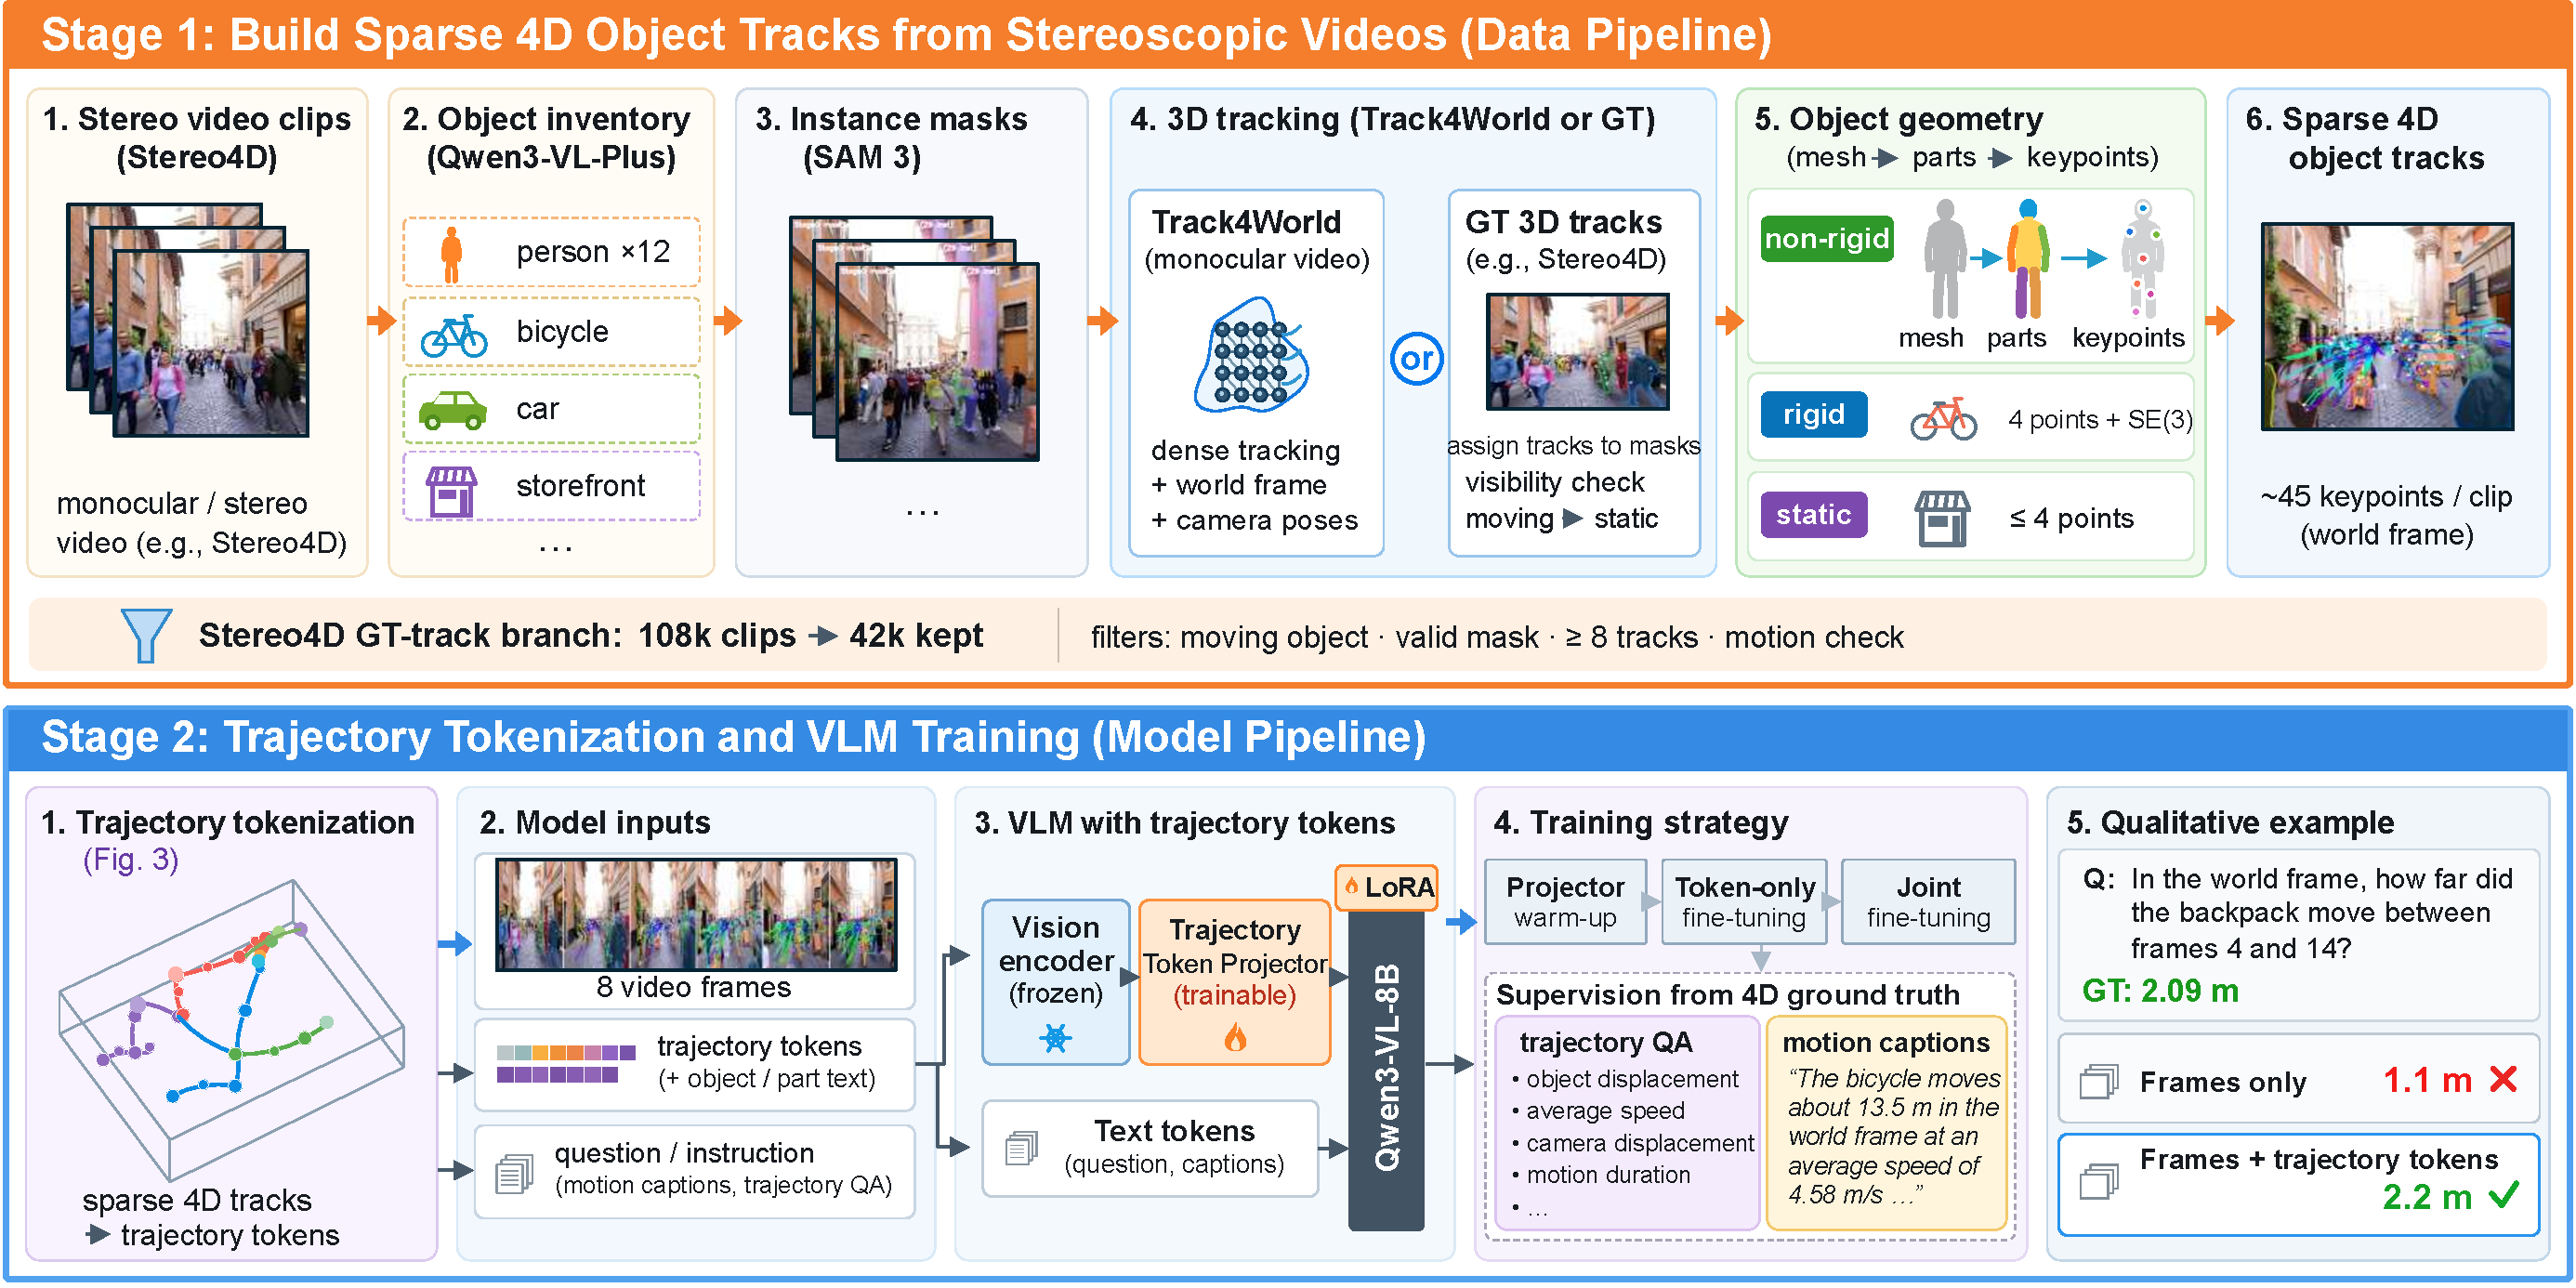
\includegraphics[width=\linewidth]{fig2_pipeline_20260926.pdf}
\caption{\textbf{Pipeline with real video frames and reconstructed tracks.} The upper row implements the Object-Centric Track Constructor; the lower row links the Event-Aware Trajectory Tokenizer to the Trajectory-Language Adapter and its three training stages. The reported QA uses released Stereo4D tracks. In the supplied artwork, ``GT'' means released reconstructed tracks, ``ground truth'' means reconstruction-derived references, and ``average speed'' means endpoint displacement rate. Track4World is an optional branch not used in the reported QA.}
\label{fig:pipeline}
\end{figure}

% ----------------------------------------------------------------------
\subsection{Object-Centric Track Constructor}
\label{sec:repr}

Figure~\ref{fig:pipeline} (top) summarizes how a video clip is converted into
\emph{sparse 4D object tracks}.
We first obtain per-object masks and dense 3D tracks with visibility and camera poses. All reported TrajQA-B results use Stereo4D's released tracks; Track4World~\citep{luTrack4WorldFeedforwardWorldcentric2026} is an optional path for other monocular videos that is not evaluated in the downstream QA results. For non-rigid objects, SAM 3D Objects~\citep{sam3dteam2025sam3d3dfyimages} reconstructs an object mesh that is partitioned into semantic parts by PartSAM~\citep{zhuPartSAMScalablePromptable2026};
representative surface keypoints are then selected and associated with the corresponding dense tracks. The complete extraction pipeline, including object discovery with Qwen3-VL-Plus,
mask propagation with SAM~3~\citep{ICLR2026_e0982cbc}, mesh reconstruction, and keypoint sampling and association, is detailed in Appendix~\ref{app:pipeline}.

The resulting representation is object-centric, part-aware, and metric. A non-rigid object uses sparse keypoints assigned to semantic parts; a rigid object uses four reference keypoints and a per-frame pose $(\mR_i,\vt_i)\in SE(3)$ estimated from its tracks; and a static object uses up to four points. For object $o$ with $K_o$ keypoints, the module returns positions $\tX_o\in\R^{K_o\times T\times 3}$, visibility $\mV_o\in\{0,1\}^{K_o\times T}$, a part index for each keypoint, and a text label. Here $T$ is the number of frames, $\mR_i\in SO(3)$ is a rigid rotation, and $\vt_i\in\R^3$ is its translation. Camera poses and timestamps are stored alongside the object tracks. All coordinates are in the reconstructed world frame, so object and camera motion can be distinguished. A scene contains 44.8 selected keypoints on average (20.7 on moving objects), rather than hundreds of dense tracks per object.

% ----------------------------------------------------------------------
\subsection{Event-Aware Trajectory Tokenizer}
\label{sec:token}

\begin{figure}[t]
\centering
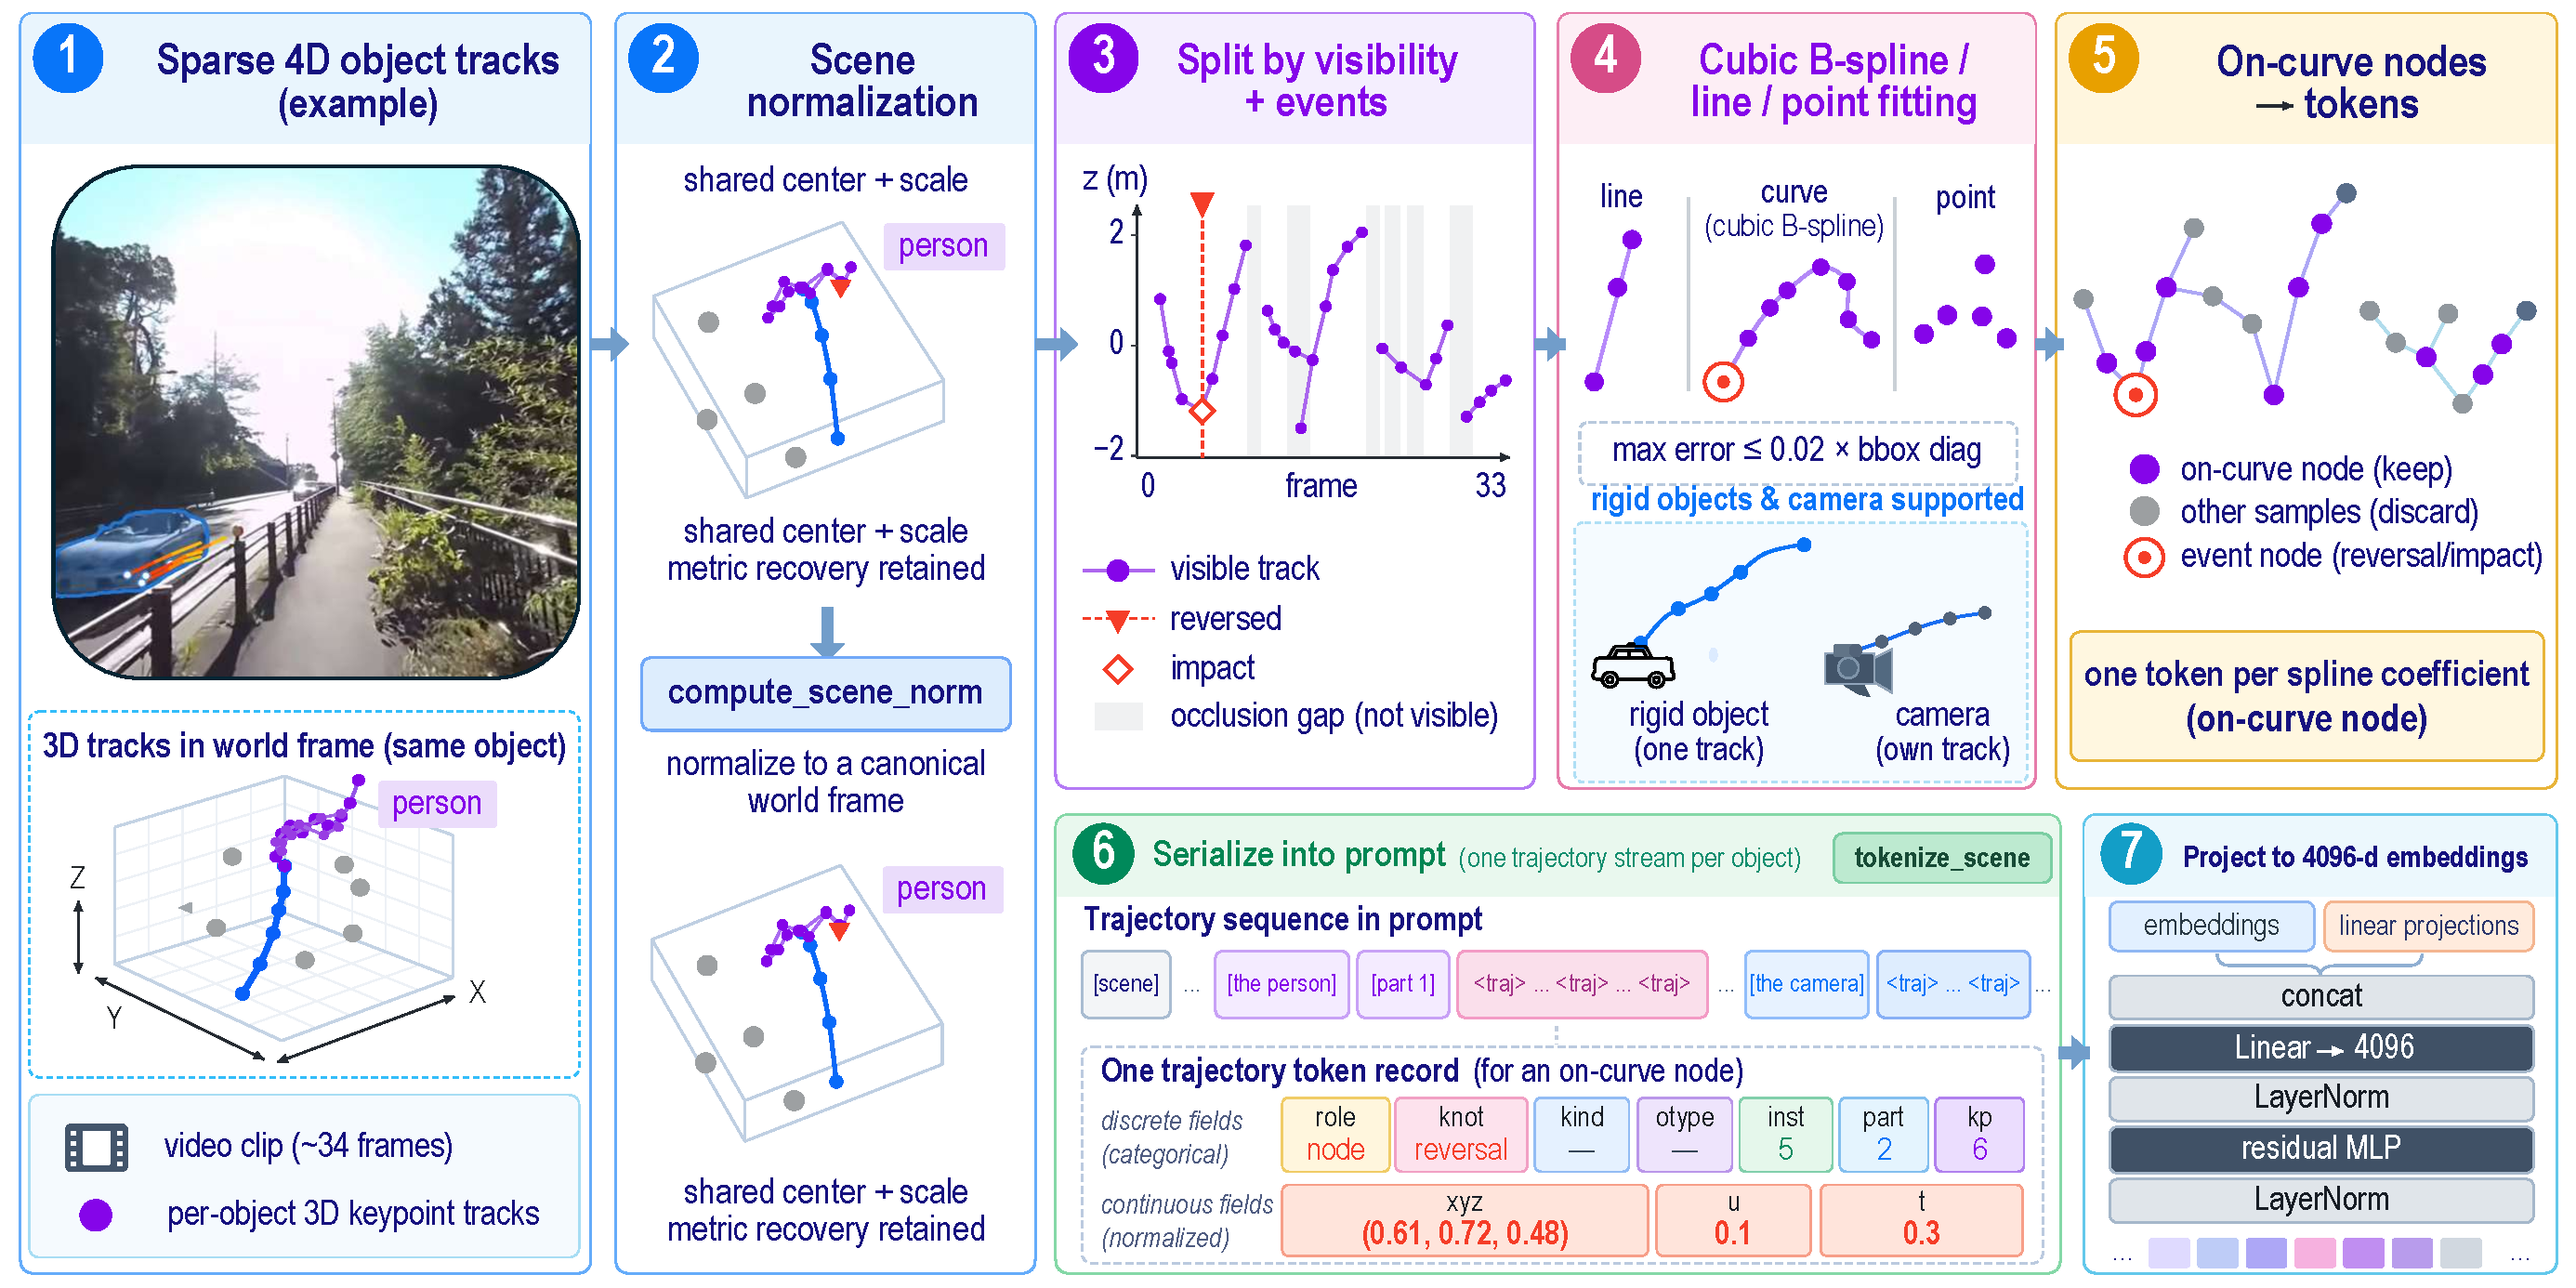
\includegraphics[width=\linewidth]{fig3_tokenization_editable.pdf}
\caption{\textbf{From a keypoint track to trajectory tokens} (one pedestrian keypoint). The scene is normalized; visible runs are split at motion events; spline pieces are fitted with a target error of $0.02$ times the trajectory bounding-box diagonal. Fitted on-curve nodes are serialized by object and part with text labels and projected into the LLM embedding space. A small fraction of pieces cannot meet the target under the node budget (Appendix~\ref{app:tokenization}).}
\label{fig:tokenization}
\end{figure}

\paragraph{Normalization and segmentation.}
All visible keypoints of a scene are shifted by their centroid $\boldsymbol{\mu}\in\R^3$ and scaled by the maximum radius $s>0$ into the unit sphere, $\tilde{\vp}=(\vp-\boldsymbol{\mu})/s$; $(\boldsymbol{\mu},s)$ are emitted as the scene header, so a metric position is recoverable as $\vp=s\tilde{\vp}+\boldsymbol{\mu}$.
A track is fitted only on its maximal visible runs: an occlusion gap is recorded explicitly rather than silently interpolated.
Within a run we detect motion \emph{events} on the inter-frame displacements: a direction change exceeding $90^\circ$ when both steps exceed a noise floor (called a reversal in the token vocabulary), or a peak in discrete acceleration (called an impact). We split the run at these event frames.
Consecutive pieces include the same observed event frame, but separate smoothing fits need not interpolate it exactly. Splitting permits a local change of direction or acceleration that a single global smooth fit might attenuate; its benefit for QA remains to be isolated experimentally.

\paragraph{Target-error fit.}
For observed frames $f_0<\dots<f_{m-1}$, let $u_i=(f_i-f_0)/(f_{m-1}-f_0)$ and fit a cubic B-spline to normalized positions $\tilde{\vp}_i$:
\begin{equation}
\mB(u)=\sum_{h=1}^{n} N_{h,3}(u;\boldsymbol{\xi})\,\boldsymbol{\beta}_h,\qquad
\max_i\|\mB(u_i)-\tilde{\vp}_i\|_2\leq\varepsilon=\alpha d,\quad \alpha=0.02.
\label{eq:fit}
\end{equation}
Here $n\leq12$ is the coefficient count, $N_{h,3}$ is the cubic basis on knot vector $\boldsymbol{\xi}$, $\boldsymbol{\beta}_h\in\R^3$ is a control point, and $d$ is the bounding-box diagonal of the object's normalized visible path. Adaptive knots allocate more nodes to harder motion. The sampled bound holds for 99.82\% of pieces; the rest retain their best fit and are counted as failures (Appendix~\ref{app:tokenization}).

\paragraph{On-curve nodes as tokens.}
For knot values $\xi_l$, the Greville parameter $\tau_h=(\xi_{h+1}+\xi_{h+2}+\xi_{h+3})/3$ yields the on-curve sample $\mB(\tau_h)$, unlike an off-curve spline control point. We serialize one node per coefficient with its mapped physical timestamp and a smooth, event, or endpoint flag. The question generator linearly interpolates these records to obtain a decoded path $\hat{\vp}(t)$ and checks its answers against the references (Gate~0). The LLM does not receive the knot vector, so the fit bound in Eq.~\ref{eq:fit} is not an error bound on $\hat{\vp}(t)$; separate event-side fits may also disagree at their shared time. Appendix~\ref{app:tokenization} details this distinction. Rigid objects fit translation and rotation jointly on shared knots; their keypoints follow $\vp_j(t)=\mR_t\tilde{\vr}_j+\vc(t)$, where $\tilde{\vr}_j\in\R^3$ is a reference point, $\mR_t\in SO(3)$ is rotation, and $\vc(t)\in\R^3$ is translation. The camera is appended as a rigid pseudo-object.

\paragraph{Serialization.}
Each record has seven discrete fields (role, knot type, kind, VLM type, instance, part, keypoint) and three continuous fields (3D value, normalized clip time, absolute seconds). A scene header stores $(\boldsymbol{\mu},s)$; objects follow with text category and part labels adjacent to their trajectory placeholders, and the camera comes last. A clip uses a median of 165 trajectory tokens against 1,152 visual tokens from eight frames. Training caps the stream at 512 records while keeping structural and event nodes.

\subsection{Trajectory-Language Adapter}
\label{sec:train}

\paragraph{Trajectory Token Projector.}
The projector (Fig.~\ref{fig:tokenization}, right) maps every token independently. Let $d_1,\ldots,d_7$ denote its seven discrete field values; $\vx\in\R^3$ is its position, rotation, reference point or gap value, $u\in[0,1]$ is normalized clip time, and $t$ is physical time in seconds. Learned tables $\mE_k$ embed discrete fields, learned matrices $\mW_{\vx},\mW_u,\mW_t$ project continuous fields, and binary gates $g_{\vx},g_u,g_t$ mark fields present in this token. A learned fusion matrix $\mW_{\mathrm f}$ and bias $\vb_{\mathrm f}$ precede layer normalization (LN) and a residual multilayer perceptron (MLP):
\begin{align}
\vh&=\mW_{\mathrm{f}}\big[\mE_1(d_1);\dots;\mE_7(d_7);\;g_{\vx}\mW_{\vx}\vx;\;g_u\mW_u u;\;g_t\mW_t t\big]+\vb_{\mathrm{f}},
\label{eq:projector}\\
\vz&=\mathrm{LN}\big(\vh'+\mathrm{MLP}(\vh')\big),\qquad \vh'=\mathrm{LN}(\vh),\nonumber
\end{align}
with 85.93M parameters in total.
Here $\vh$ is the fused field representation, $\vh'$ its normalized value, and $\vz$ the output token embedding.
It contains no attention, convolution or pooling, so every relation between trajectories is formed inside the LLM.
Its outputs replace the placeholder embeddings by a masked scatter into the LLM's input embeddings; trajectory tokens are otherwise treated as text (ordinary 1-D positions on all rotary axes) and never pass through the vision encoder.

% ----------------------------------------------------------------------

The backbone is Qwen3-VL-8B-Instruct with frozen vision and base weights. We train the projector and language-model LoRA adapters~\citep{huLoRALowRankAdaptation2021} by next-token cross-entropy on generated evidence and answer text. Stage~1 warms up the projector on rule-generated motion captions with the base model frozen; Stage~2 learns token-only QA with the projector and LoRA; Stage~3 restores frames and drops them independently with probability 0.2 while keeping tokens. This sequence first teaches the new interface to express motion and then adapts it to metric questions. All three training stages exclude QA evaluation scenes; stages~2 and~3 additionally use source-video-disjoint QA splits. A stage-1 source-video audit remains to be documented (Appendix~\ref{app:training}).
